\documentclass[twocolumn, 9pt]{article}
\usepackage{comment}
\usepackage{float}
\usepackage{appendix}
\usepackage{cite}
\usepackage{cuted}
\usepackage{fullpage} 
\usepackage[english]{babel}
\usepackage[utf8]{inputenc}
\usepackage{amsmath}
\usepackage{graphicx}
\usepackage[makeroom]{cancel}
\usepackage{multirow}
\usepackage{multicol}
\usepackage[T1]{fontenc}
\usepackage[utf8]{inputenc}
\usepackage{authblk}
\usepackage{xcolor}
\usepackage{soul}
\usepackage{listings}
\usepackage{rotating}
\usepackage{pdflscape}
\usepackage{wrapfig}
\usepackage[utf8]{inputenc}
\usepackage{listings}
\usepackage{natbib}
\usepackage{hyperref}

\begin{document}

\title{Estimating Parameters of a Coupled ODE}

\author[1]{Eliot Heinrich}
\author[2]{Alexander Looi} 
\affil[1]{University of Vermont, Undergraduate}
\affil[2]{University of Vermont, Graduate}

\twocolumn
\maketitle
\section*{Abstract}
\indent{} Models similar to the original Lotka-Voltera predator-prey models can be useful tools for understanding systems. But, a model is only as useful as its ability to describe a system. In the case of first order ordinary differential equation (ODE) models users need an accurate understanding of the parameters that make up the model as well as the model construction itself. Here we test our understand of our own predator-prey ODE model and how its parameters changed across different data sets by optimizing its parameters to two different sets of data using 5 different algorithms; two gradient descent, a single objective and two MO algorithms. The synthetic data was noised at four different levels and the real experimental data represented four different environmental conditions. Here, the variable model parameters solutions generated by these optimizing algorithms should tell us how parameter variables vary across differing amounts of noise, and different environmental conditions.
\section{Introduction} 
\indent{} The goal of mathematical models are to describe real properties and dynamics of the natural world. The original Lokta-Volterra Ordinary Differential Equations (ODE) aimed to describe the interactions of predator and prey through numerical values that describe specific properties in the system. Many experiments and observational studies have provided evidence that this family of equations can describe the dynamics of real world predator prey interactions \cite{fussmann_crossing_2000, yoshida_rapid_2003, huffaker_experimental_1958, utida_cyclic_1957}. Additionally, many of these same studies were able to build ODE models that related simple behaviors and characteristics of predator and prey to the overall dynamics of the system. Take for example a parameter like the growth rate of a population of prey. Predator-prey models built using this parameter showed that a two-species predator-prey system could transition from stable coexistence, to stable limit cycles, and finally amplitudes with high extrema which resulted in extinction as prey growth rate was tune from low to high. \\

\indent{} It is known how this kind of bottom up forcing can affect dynamics of the predator and thus the overall dynamics of a system \cite{smith_rosenzweig-macarthur_nodate, mccauley_physiological_1990, mccauley_growth_1990, mccauley_cyclic_1987, mccauley_large-amplitude_1999}. Less attention is given to the effect of tuning predator behavior (i.e. top down forcing). Some studies have attempted to alter aspects of just predator efficacy in consuming prey. For example, Luckinbill \cite{luckinbill_coexistence_1973, luckinbill_effects_1974} was able to alter the encounter rate of predator and prey, both aquatic ciliates, by increasing viscosity of their medium. In this study we use four salinity concentrations ($3 gL^{-1}$, $16 gL^{-1}$, $35 gL^{-1}$, $45 gL^{-1}$) of the predator and prey media to tune the feeding rate of the predator, a marine rotifer (Unpublished Data). 

\indent{} In this system, the predator had a narrower optimal growth range across the aforementioned salinity ranges compared to its algal prey \cite{snell_effect_1986, sarma_effect_nodate, miracle_salinity_nodate}. Additional experiments documented differing dynamics between predator and prey among the four experimental salinities (unpublished data).
Below are a set of ODEs were used in an attempt to predict describe our predator prey system. \\
\begin{align}
    FcN = \frac{\beta_C*N}{(K_c+N)} \\
    FbC = \frac{\beta_R*C}{(K_r+C)} \\
    \frac{dN}{dt}=\delta*(80-N)-FcN*C \\
    \frac{dC}{dt}=FcN*C-(FbC*\frac{R}{e})-\delta*C \\
    \frac{dR}{dt}=FbC*R-(\delta+m)*R 
\end{align}

\indent{} Here, $N$, $C$, and $R$ are the concentrations of nitrogen, chlorella (prey), and rotifers (predator) respectively. $\beta_C$ is the growth rate of the prey and $\beta_R$ is the growth rate of the predator. $K_c$ and $K_r$ are the half saturation constant of the prey and predator respectively \cite{fussmann_crossing_2000}. Lastly, $\delta$ is the flow through rate of the system (i.e. the dilution rate) and $m$ is the death rate of the predator. $\frac{dN}{dt}$, $\frac{dC}{dt}$, $\frac{dR}{dt}$ describe the change in density of nitrogen, prey, and predator respectively. With these coupled ODEs we can describe the predator-prey system. According to our original hypothesis we expect that the $\beta_R$ parameter to be the parameter that was responsible for altering dynamics among the different salinities. However, initial model simulations using experimentally derived parameters, and parameters fit using basic gradient descent algorithms produced poor fitting and unrealistic solutions.  

\indent{} Models like the one described above, need to accurately portray the data they aim to represent if researchers are to say that they understand the system. Our initial gradient descent and experimentally derived results, suggests our understanding of the system is flawed. To gain a better understanding of how parameters in this system of equations interact, we optimised the aboved equation to the four salinities that comprise our experimental data using three techniques: 1) Single-Objective Differential Evolution (SODE), 2) Non-dominated Sorting Algorithm II (NSGAII), and 3) Spatial Pareto Evolutionary Algorithm 2 (SPEA2) \cite{deb_fast_2002, zitzler_spea2:_nodate, rocca_differential_2011}.

\indent{} After optimizing multiple times and getting a suite of viable solutions (assuming that this problem exhibits non-uniqueness) we see if there are 1) multiple parameter sets that can accurately describe a data set given our current model of the system, 2) how the parameter sets may vary if the problem is non-unique, and 3) tell how sensitive each parameter is at the four different salinities. 

\section{Methods}

\indent{} The system of ODEs was optimized over the predator and prey abundance over time. Thus, to measure how well the simulations of a parameter set matched the data we used a version of the mean squared error (MSE) for both predator and prey. However, this poses a slight problem because this means we have two values or objectives in a fitness function. Three techniques with two different types of objectives were used to optimize the system of ODEs. The SODE technique is a single-objective, meaning there was only one value that needed to be optimized. NSGAII and SPEA2 are multi-objective (MO) techniques, meaning these algorithms optimized over two values. This resulted in us using two different fitness functions. 

\subsection{Fitness Functions}
\begin{table*}[t]
    \caption{Parameter bounds used in all optimization techniques discussed in this paper. Included are the sources for the parameter bounds and initial estimates at the four different experimental salinities (these are unpublished data based on experiments). All initial estimates (right side of table 1) are experimentally derived or obtained from \cite{fussmann_crossing_2000}} 
    \hrule
    \begin{tabular}{c c}
        \hline
    	\label{table:Bounds} % table for the Bounds
        	\begin{tabular}{c c c}
        	Parameter & Bound & Source \\
        	\cline{1-3}
        	$\beta_C$ & 1.0 - 25.0 & \cite{fussmann_crossing_2000, wen_biological_2005}\\
            $K_c$ & 1.0 - 10.0 & \cite{laliberte_regulation_1989, ahmad_nitrogen_1984}\\
            $e$ & 0.01 - 0.5 & \cite{malekzadeh_viayeh_population_2010, snell_effect_1986}\\
            $m$ & 0.0 - 1.0 & Unpublished Data\\
            $\beta_R$ & 1.0 - 25.0 & \cite{doohan_energy_1973, peredo-alvarez_combined_nodate}\\
            $K_r$ & 1.0 - 50.0 & \cite{cheng_effects_2011, lowe_evidence_2005, yufera_factors_nodate}\\
    	\end{tabular}
    	&
    	\label{table:Bounds} % table for the Bounds
        	\begin{tabular}{c c c c c}
        	Parameter & 3$gL^{-1}$ & 16$gL^{-1}$ & 35$gL^{-1}$& 45$gL^{-1}$\\
        	\cline{1-5}
        	$\beta_C$ & 3.3 & 3.3 & 3.3 & 3.3\\
            $K_c$ & 4.3 & 4.3 & 4.3 & 4.3\\
            $e$ & 0.25 & 0.25 & 0.25 & 0.25\\
            $m$ & 0.3 & 0.56 & 0.2 & 0.3\\
            $\beta_R$ & 1.00 & 2.16 & 2.4 & 1.00\\
            $K_r$ & 15 & 15 & 15 & 15\\
    	\end{tabular}
    \end{tabular}
    \hrule
\end{table*}
\indent{} In this study, the horizontal distance between the simulated data produced from a set of parameter estimates and the actual (experimental) data was minimized. There are two species (the predator and prey), thus we need fitness functions that can appropriately capture the error between the simulations and the data of both, and still guide our algorithms to the best solution. Additionally, we only care about the absolute deviation from data and want to severely penalize large deviations; this is why we used MSE.

\indent{} For the SO fitness function we added the errors of the predator and the prey together. However, there is the potential for the MSE of the prey to dominate the fitness function because the numerical units of the prey are greater than the predator (millions of individuals vs several). Thus, to avoid one species dominating the fitness function when combining the predator and prey MSE we used the Root Mean Squared Error (RMSE) divided by the mean of the data set.

\begin{align}
    MSE=\frac{1}{n}\sum_{i=1}^{n} (Y_i - Y)^2 \\
    RMSE=\frac{\sqrt{\frac{1}{n}\sum_{i=1}^{n} (Y_i - Y)^2}}{mean(Y)}
\end{align}

\indent{} By square rooting the MSE value, we obtain the original units of the predator and prey error. Then by dividing by the mean of the data, we can normalize the absolute value of the MSE, this gives us a normalized unit-less number to use as a fitness value which were then added together to be used in the SO algorithms. In this final form the prey will not dominate the fitness function unless simulations significantly deviate from the data. Lastly, for both SPEA2 and NSGAII we used the RMSE values as described before, however, rather than adding them together we simply passed them directly as the two objectives to be optimized for. By using the RMSE for the MO problems we can still compare MO errors to the SO errors.

\subsection{Experiments:}

\intdent{} As a control we compared the results of the GAs to two gradient descent algorithms: Nelder-Mead (NM) and the Limited Memory Broyden–Fletcher–Goldfarb–Shanno (BFGS). We ran the gradient descent algorithms at 30 different random seeds to get a variety of solutions. The SOBE were run at the same 30 random seeds with a population of 100 individuals and were allowed to run until the function self terminated. The best individual at the end of these thirty runs was taken as data to explore how parameters vary among the best solutions.

\indent{} The MO algorithms were run for 100,000 generations with a population of 100 individuals. The best 30 individuals (top 30 individuals along the Pareto front) of the final Pareto set of solutions were taken as best solutions and these parameter sets were used as the data to explore how parameters vary among the best solutions. Lastly, for all algorithms used, the range of acceptable parameter values were bounded so that parameter values estimated by our algorithms remained plausible, or at least within the range observed in the original studies and literature (for reference see table \ref{table:Bounds}). 
% table about the parameter bounds and the initial values used that were derived from experiments.
% table 1 Parameter Bounds and Sources


\section{Results}
\subsection{Representative Plots}
% Talk about Representative runs here:
\indent{} The Gradient Descent methods did not produce viable solutions partly because they always found the same local minimum at all random seeds (Figure \ref{fig:RepGenData}). Additionally, those methods consistently had the highest RMSE values in addition to finding solutions that did not fit the generated data well. Parameter sets for these two algorithms generated predator prey dynamics that stayed more or less constant (i.e. straight lines through time) despite the clear cyclic dynamics in the generated data. \\

\begin{figure*}[t]
    \centering
    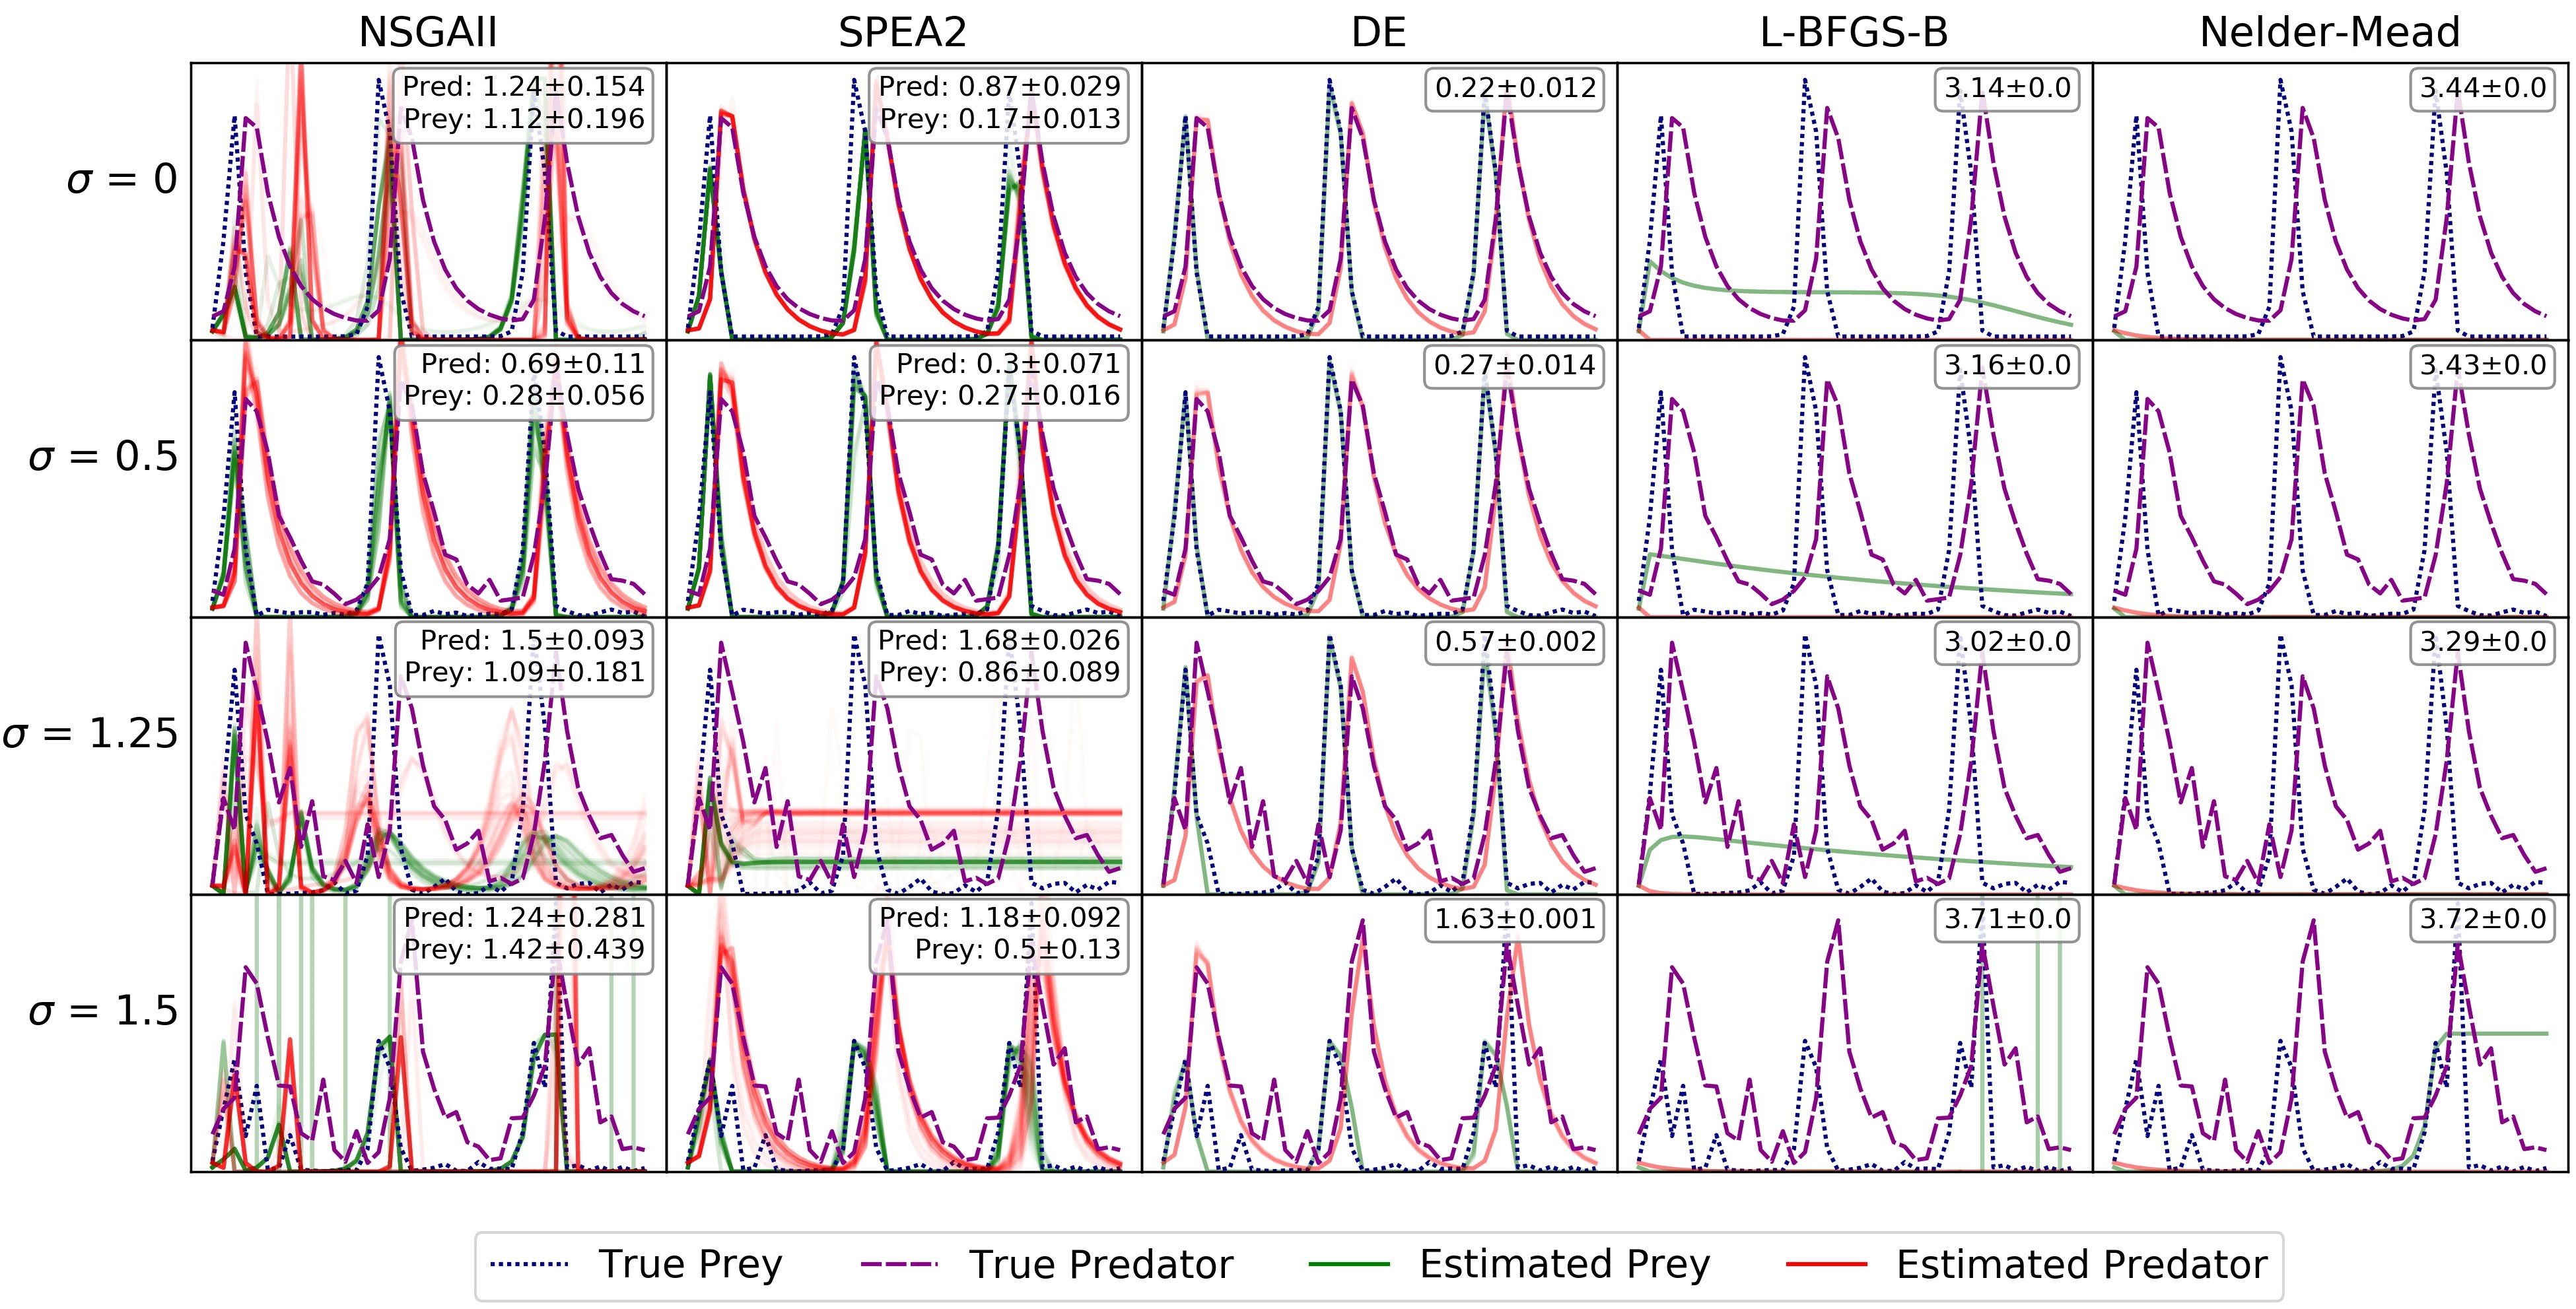
\includegraphics[width=\textwidth]{RepPlotsGenData.jpeg}
    \caption{Simulations from the top 30 parameter solutions generated by each algorithm (green solid line for prey, red solid line for predator). The simulations are superimposed under the generated data (what was being fitted to), dotted blue lines represent true prey values, dashed magenta line for true predator. Each row of figures indicates the value $\sigma$ data was noised. Inset for each figure is the mean and $\pm$ the standard deviation of the RMSE from the top 30 solutions. For the MO algorithms the mean and $\pm$ the standard deviations of the two objectives are shown.}
    \label{fig:RepGenData}
\end{figure*}

\indent{} Between the two MO algorithms, SPEA2 appears to find the better solutions compared to NSGAII for the generated data. SPEA2 performed much better relative to NSGAII, particularly at the highest level of noising ($\sigma = $ 1.5). Despite this, when $\sigma = $ 1.25, SPEA2 performed worse compared to NSGAII shown by the greater RMSE values for predator (prey RMSE was still lower compared to NSGAII). The dynamics generated from the SPEA2 parameters at a $\sigma = $ 1.25 were constant over time, contrary to the cyclic dynamics in the generated data. At all other $\sigma$ levels SPEA2 out performed NSGAII. The SODE consistently produced the lowest RMSE values at all $\sigma$ levels. Even if we summed the predator and prey errors from the MO algorithms, and compare them to the SODE we still see that the SODE algorithm has lower errors. In addition to these lower errors, SODE consistently had the lowest error standard deviation suggesting that it was finding similar solutions for each run, or at least parameter sets that produced similar dynamics. This can be seen in the in \ref{fig:RepGenData} (i.e. passing the "eye-test" most relative to the results of other algorithms). These plots indicate that most of these algorithms estimate parameters that generate viable solutions, even with added noise.

\indent{} Figure \ref{fig:RepRealData} show the dynamics generated from viable parameter sets found by all algorithms used in the study plotted against the experimental data. Again, the two gradient descent algorithms performed the worse in terms of mean RMSE which can be seen in the resulting simulations (figure \ref{fig:RepRealData}). All dynamics simulated by the parameter sets found by the gradient descent algorithms tended to miss entire cycles present in the data, and/or only fit to either the prey or predator. The MO and SO algorithms performed better having much lower RMSE values relative to the gradient descent methods in addition to finding solutions that visually match the experimental data better.

\indent{} In contrast to the generated data, NSGAII appears to out perform SPEA2 across most salinities both visually and in terms of the mean RMSE. SPEA2 does consistently find better solutions compared to NSGAII at $45 gL^{-1}$ (seen in the lower mean and standard deviation in the error). In some cases the MO algorithms could fit one objective well but would not fit the other objective well (figures \ref{fig:MOEAConvergence} \ref{fig:RepRealData}). We can see this in figure \ref{fig:RepRealData} looking at the SPEA2 algorithm trying to fit solutions to the $16 gL^{-1}$ data set. Here, the predator data fits well, but the solutions misses the growing cycles in the prey. In other cases the MO algorithms perform poorly as measured by RMSE and visually. For example NSGAII at $35 gL{-1}$ appears to produce flat lines near zero, and SPEA2 at $3 gL{-1}$ produced dampened cycles, when the experimental data cycles.

\indent{} Again DE out performed all other algorithms, consistently having the lowest RMSE and visually having the solutions that fit the closest to the experimental data. Additionally, because of the low mean RMSE and relatively low standard deviation in RMSE, DE consistently produced good solutions.  

% RepGenData figure here
% representative runs showing estimated data, and the real/generated Data
\begin{figure*}[t]
    \centering
    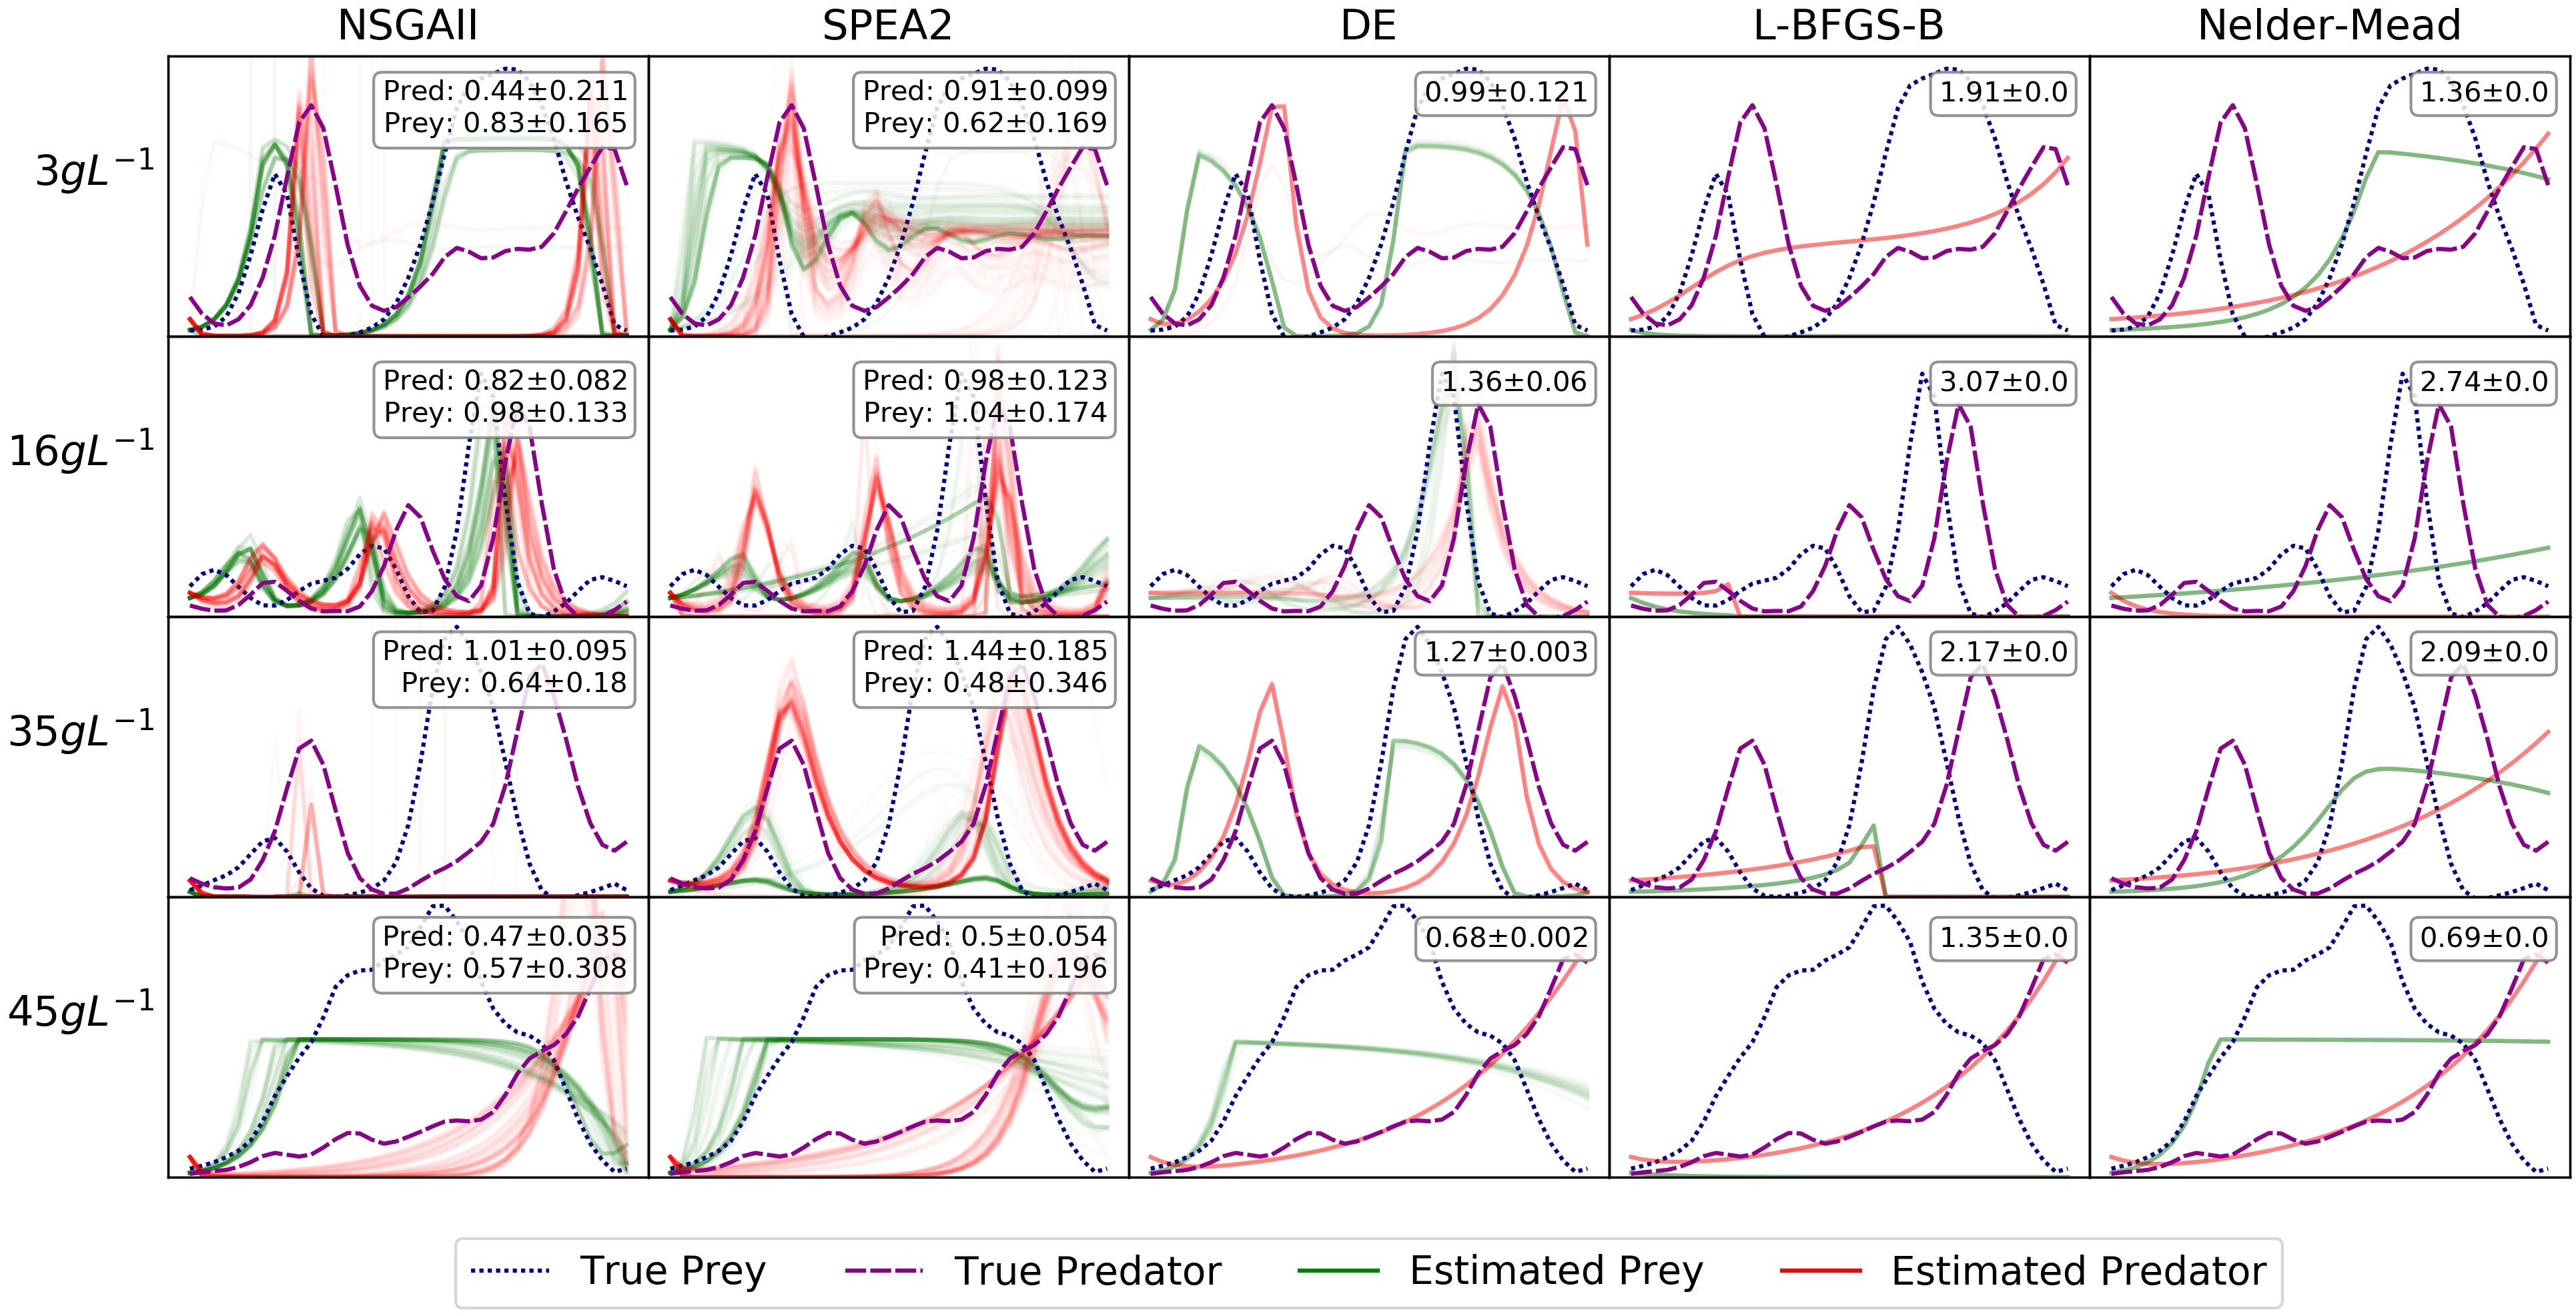
\includegraphics[width=\textwidth]{RepPlotsRealData.jpeg}
    \caption{Simulations from the top 30 parameter solutions (green solid line for estimated prey, red solid line for estimated predator) superimposed under the experimental data. dotted blue lines represent prey data, dashed magenta line for predator data. Inset for each figure is the mean and $\pm$ the standard deviation of the RMSE from the top 30 solutions. For the MO algorithms the mean and $\pm$ the standard deviations of the two objectives are shown.}
    \label{fig:RepRealData}
\end{figure*}

% could be because there are basins of attraction/local minimums in the fitness landscape that either the predator or prey will dominate. 
\subsection{Parameter Distributions}
% Talk about Parameter Distributions here 
\indent{} Figure \ref{fig:SigmaParameterSols} show the distributions for top 30 parameter solutions each algorithm when fitting for each algorithm. All algorithms produced populations of unique parameter sets relative to other algorithms across all the levels of noise (Kruskal-Wallis Test at an $\alpha$ value of 0.05). For all algorithms estimates for $e$ and $m$ were consistent across all four salinities, with the specific value of these parameters sometimes differing (i.e. at $\sigma =$ 1.25 estimated values of $m$ for SPEA2 and NSGAII were very different compared to the other algorithms). In contrast some algorithms produced a greater range of parameter values compared to other algorithms for a particular parameter. For example, DE consistently predicted larger ranges for $K_c$ compared to most other algorithms across all salinities. This is particularly interesting for DE because this algorithm produced the most consistent and low RMSE solutions for the generated data. Again, this figure shows how well DE recreated the original data. Most parameter distributions either crossed, or were close the original (blue horizontal line in figure \ref{fig:SigmaParameterSols}).

% Figure showing parameter values estimated using the Generated Data
\begin{figure*}[t]
    \centering
    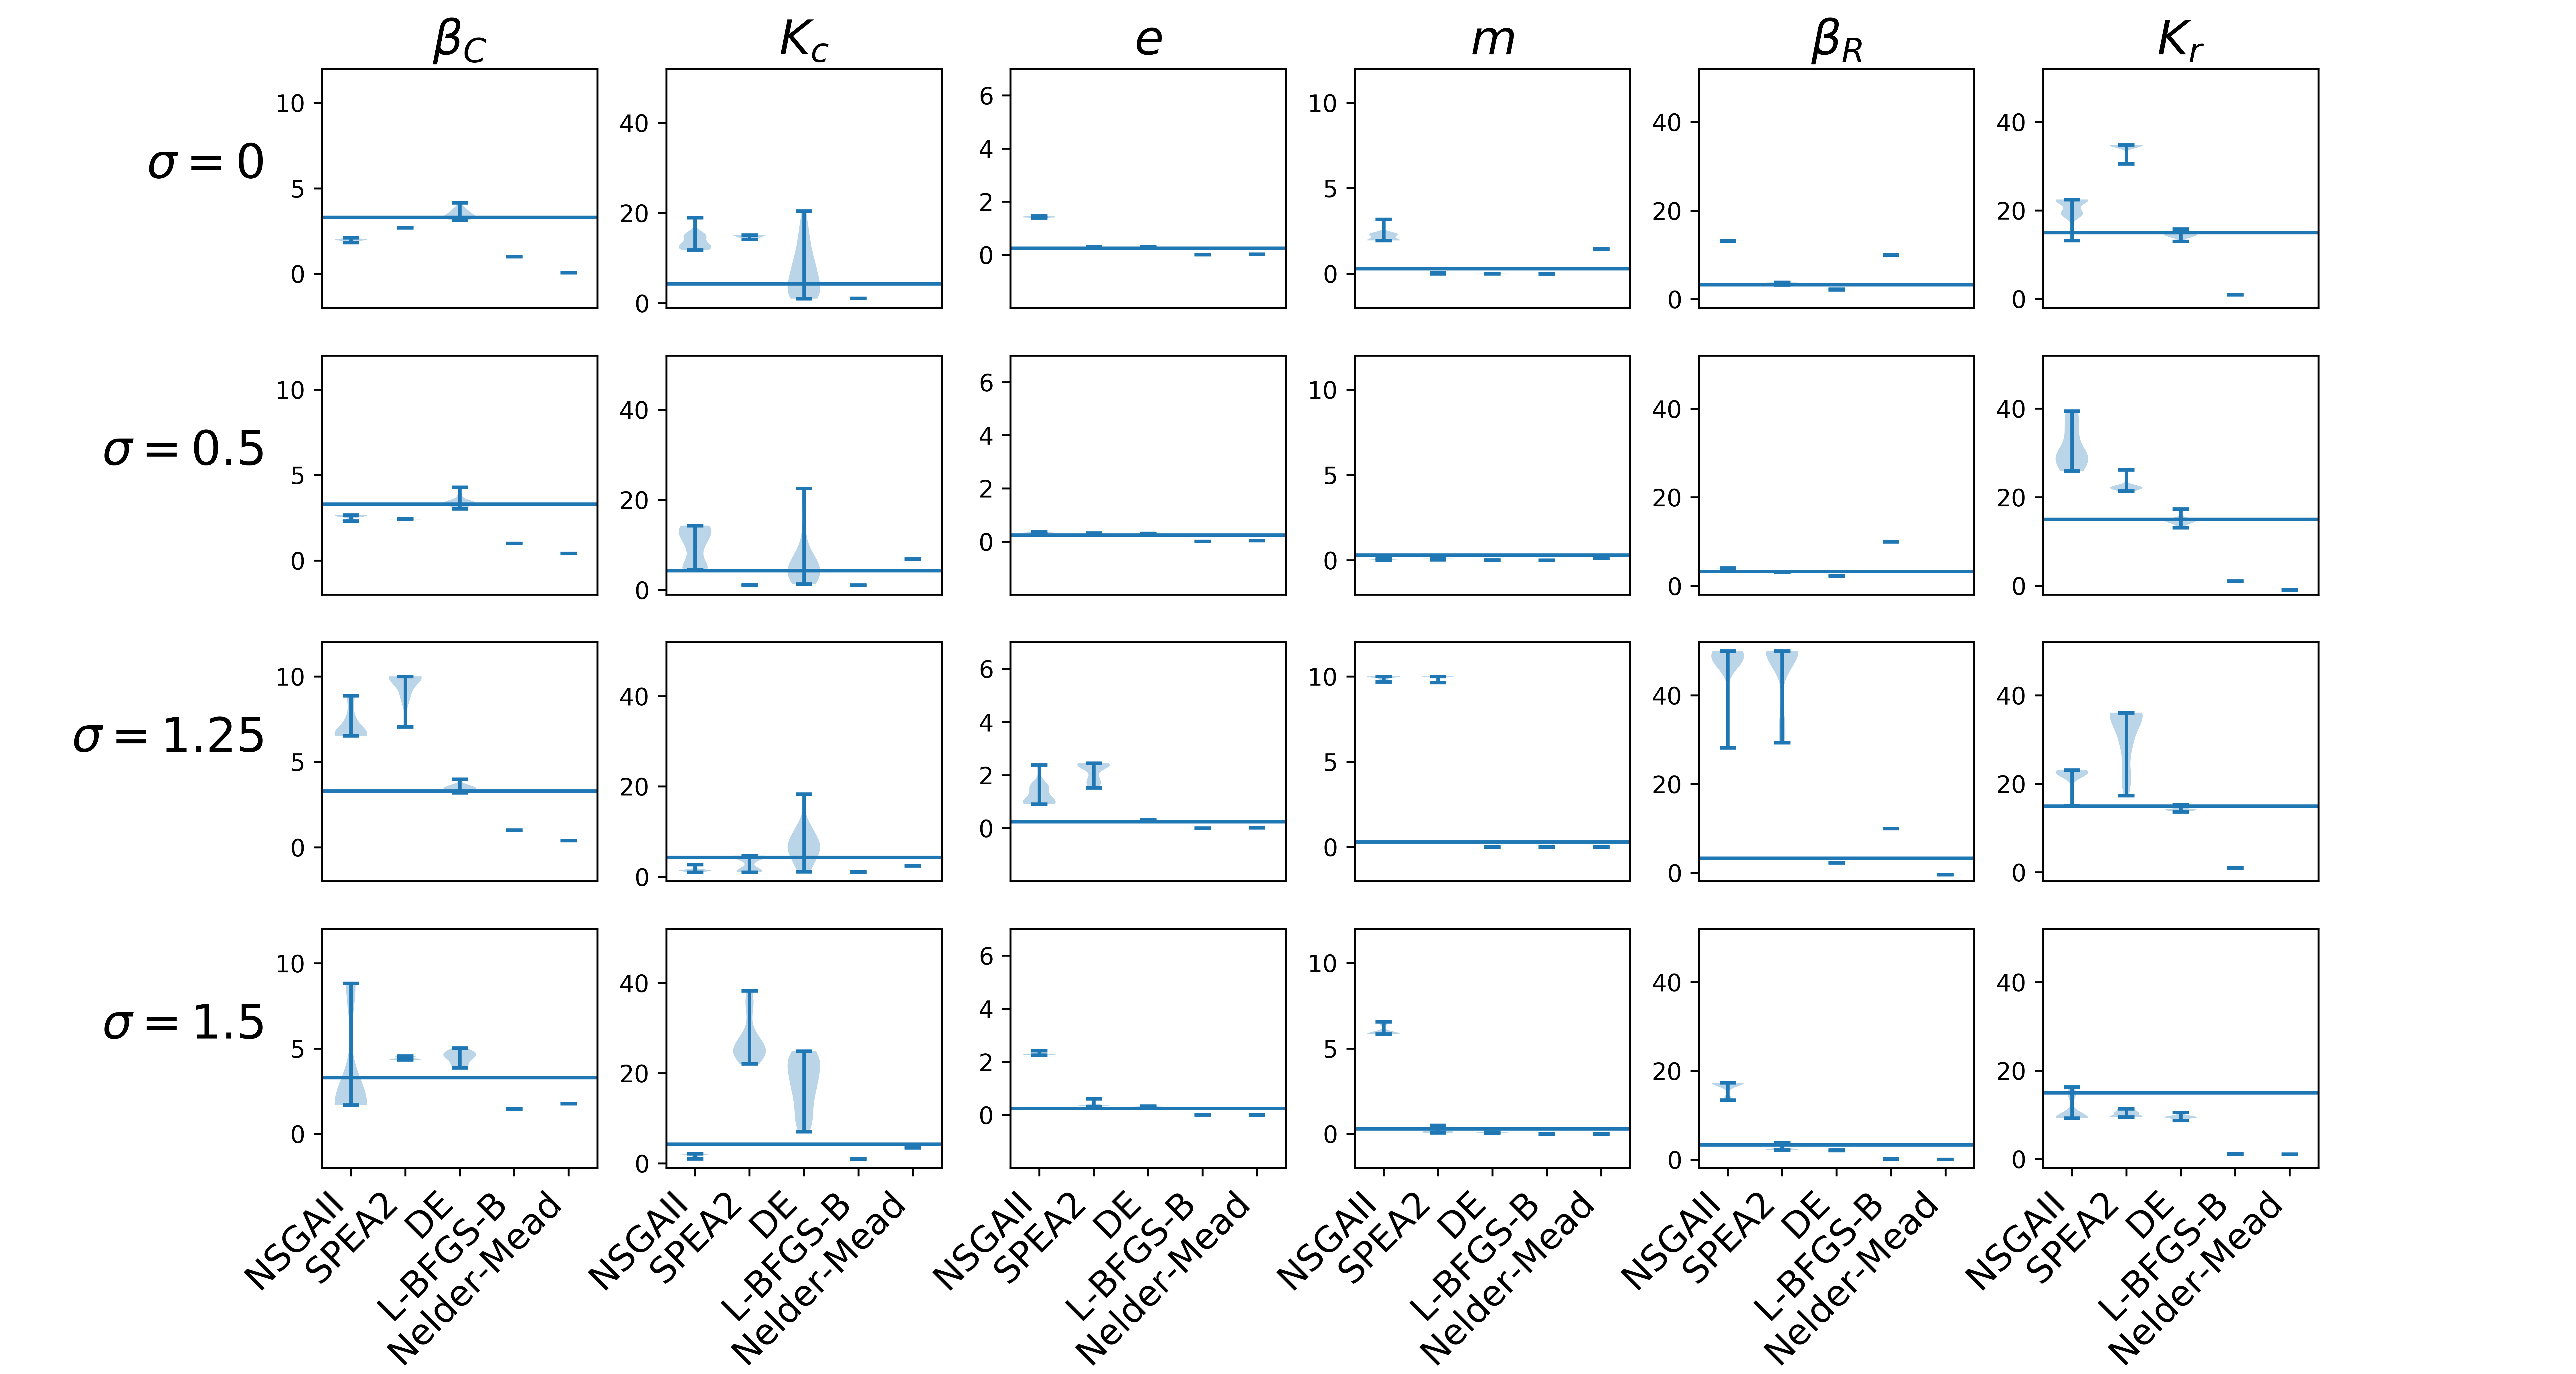
\includegraphics[width=\textwidth]{sigmaParameterFig.png}
    \caption{Parameter value distribution estimated by each algorithm, at different sigma values (i.e. different amounts of noise). Horizontal lines indicate the position the actual parameter value used to generate the original data set.}
    \label{fig:SigmaParameterSols}
\end{figure*}

Figure \ref{fig:ParameterSols} show the distributions for top 30 parameter solutions found by each algorithm when fitting to the experimental data. In contrast to figure \ref{fig:ParameterSols} there were greater ranges of parameter value estimates where some of these solutions lay at boundaries of their allowable range. No one algorithm found solutions at all of our initial parameter estimates which was expected because these solutions did not originally work. 

%  (example). However, in other case it makes sense to extend the allowable range beyond what we originally constrainted it to (example).
\begin{figure*}[t]
    \centering
    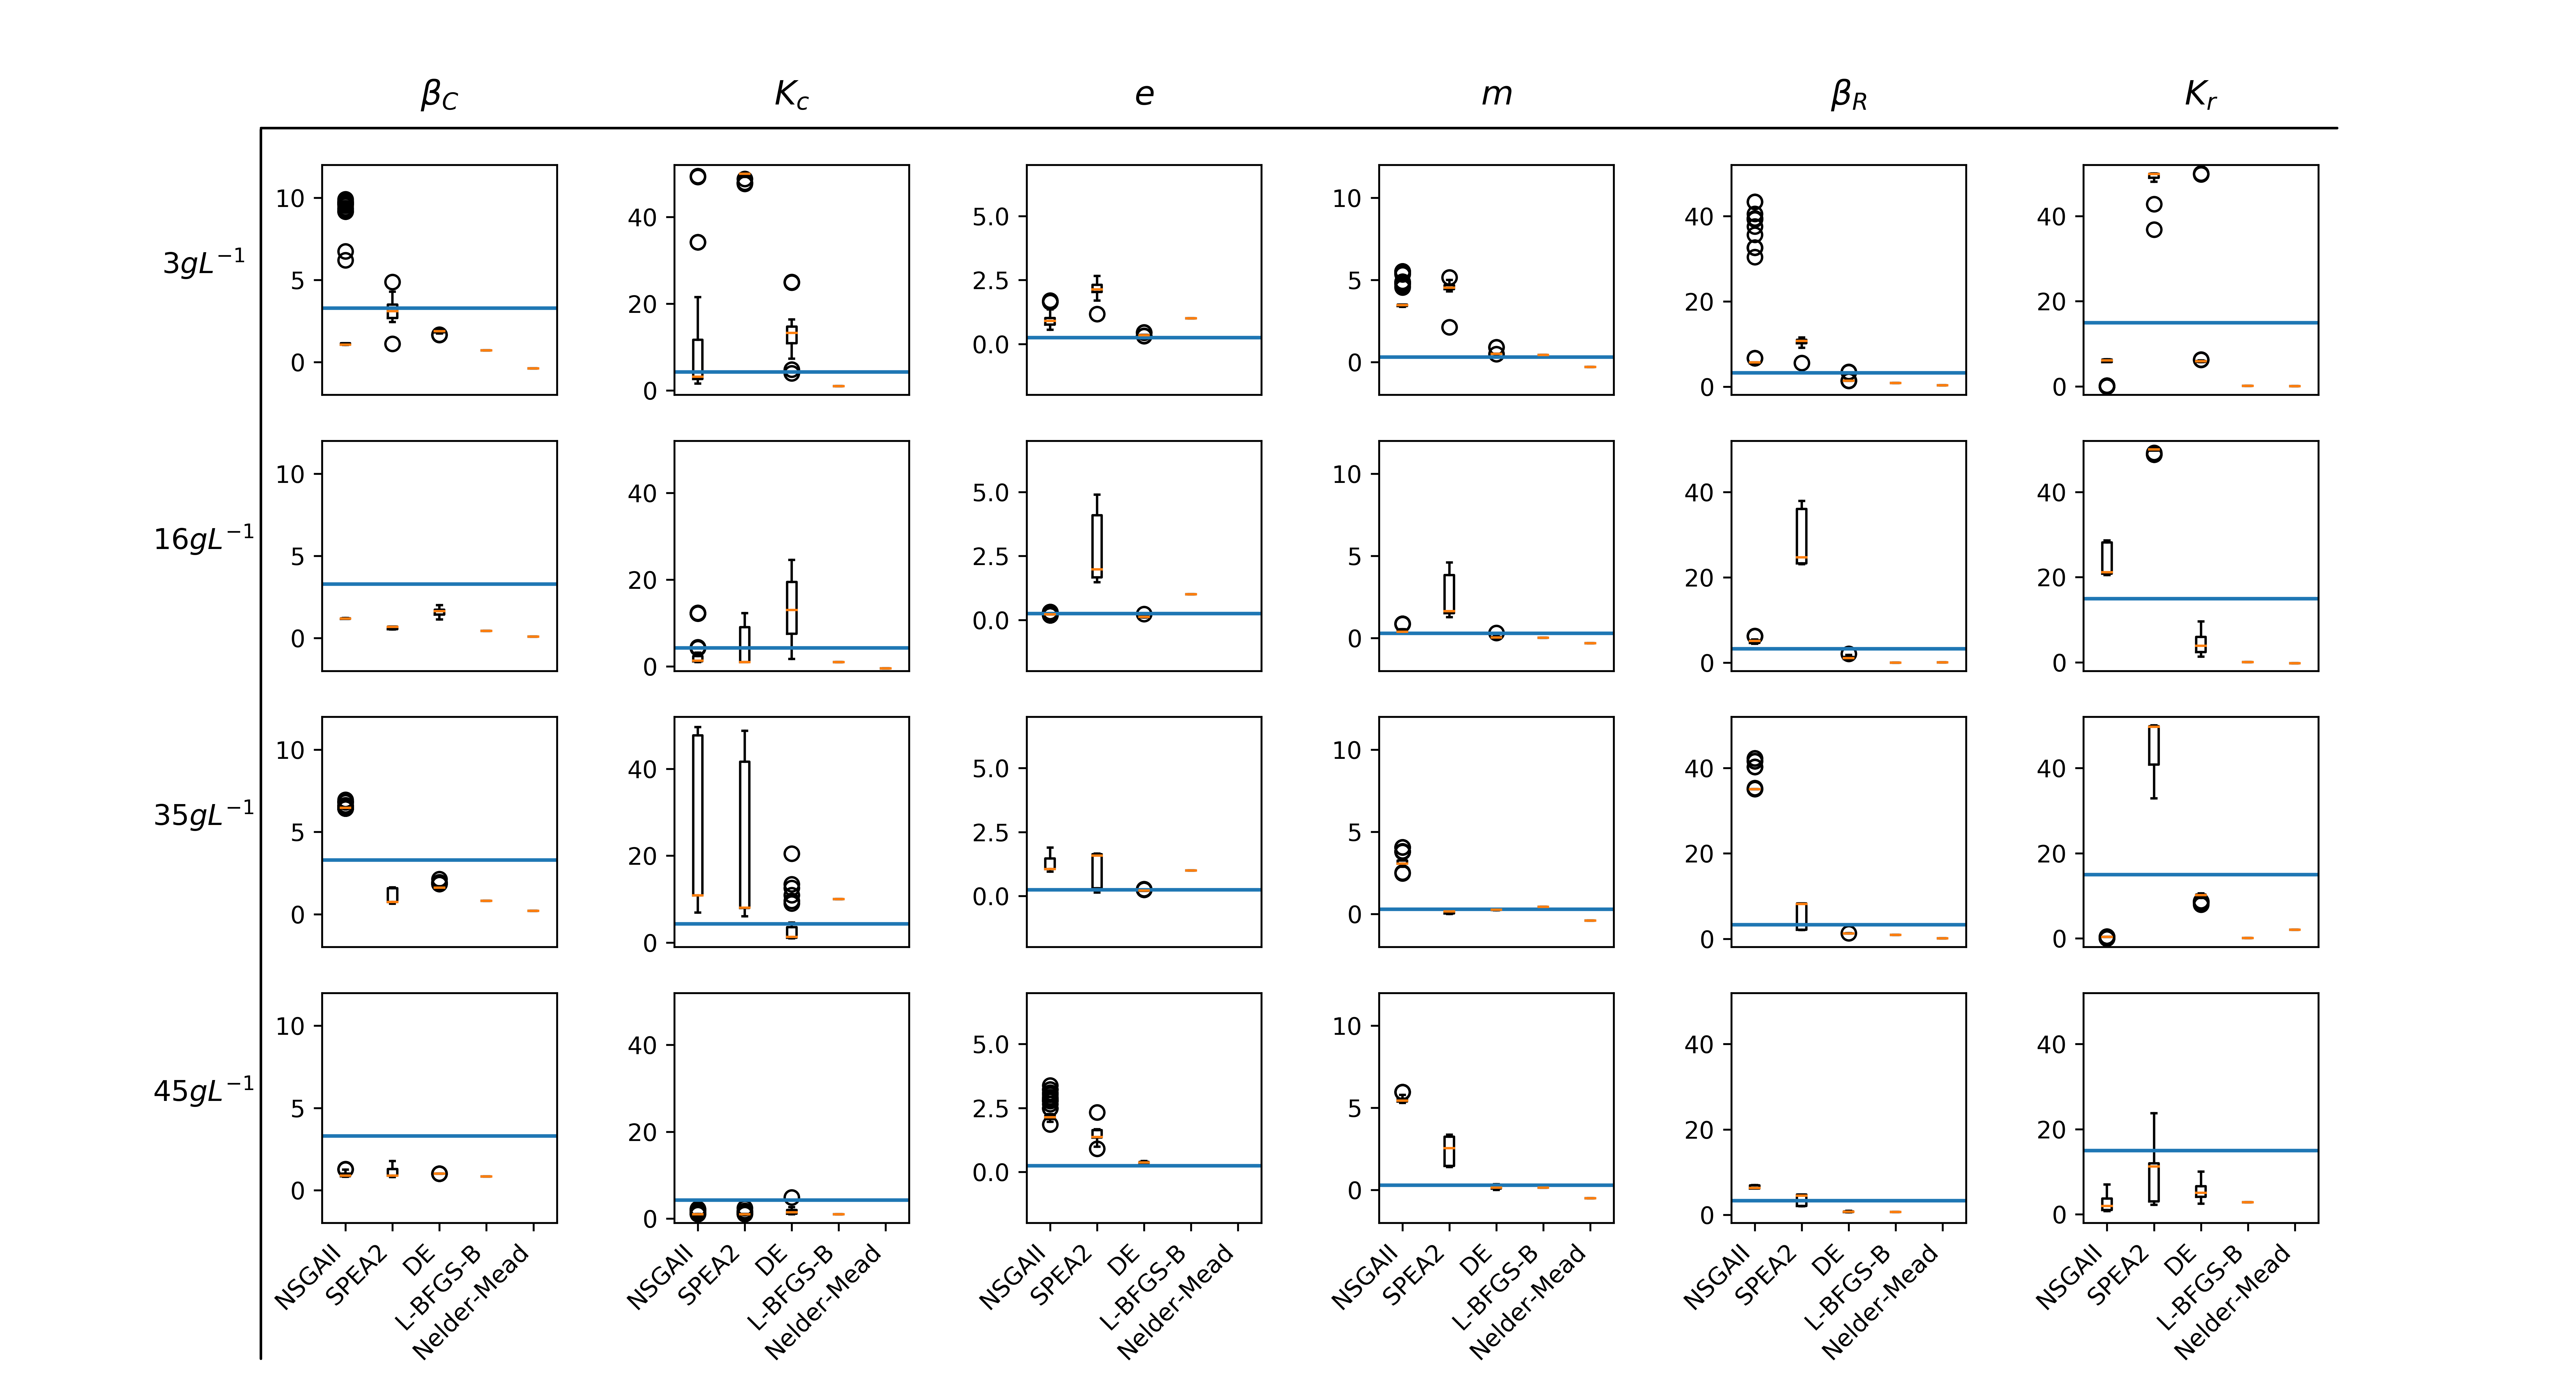
\includegraphics[width=\textwidth]{ParameterFig.png}
    \caption{Parameter value distribution estimated by each algorithm for different salinity levels. Horizontal lines indicate the position of initial estimates of the parameter values provided by in lab experiments.}
    \label{fig:ParameterSols}
\end{figure*}

\section{Discussion}
\indent{} Gradient descent methods converging on the same solutions for every random seed is somewhat surprising assuming that the fitness landscape is pocked with local minima. This appears to be the case, considering the spread of parameters generated by the other algorithms as seen in figures \ref{fig:ParameterSols} and \ref{fig:SigmaParameterSols}). This result still points to the fact that gradient descent algorithms do not explore this fitness landscape well. Because given 30 different random seeds the gradient descent algorithms all found the same poor solutions.

\indent{} Initially it was surprising that the MO algorithms did not perform better relative to SODE. However, the MO algorithms were only started at a single random seed (which was the first random seed for all other algorithms), and the top 30 solutions were taken from their respective final Perato front. In contrast, remember that DE was run at different 30 random seeds and the best solutions from those 30 individual runs were used as the best solutions. The MO optimization algorithms are slightly harder to parse and compare in this regard. One advantage of the MO optimization algorithms is that it gives us the ability to choose how we want the solutions to favor each objective. In the SO formalization the two objectives are obfuscated making it difficult to determine how the objectives interact. Thus, a future more fair comparison would be to run the MO algorithms at the same 30 random seeds as DE.

%\indent{} The range of the parameters seen in figures \ref{fig:RepGenData} and \ref{fig:RepRealData} show that there are a range of parameters that are consistent with the data. I'm not sure what you're trying to say about these two figures since they don't plot parameter values...

\indent{} Some parameters have much wider ranges relative to other parameters which suggests that the dynamics of the system is not particularly sensitive to that parameter. $K_c$ as estimated by DE is a good example of this for both the generated data and the experimental data (figures \ref{fig:SigmaParameterSols}, \ref{fig:ParameterSols}). Here DE runs on the simulated data generated solutions have greater variation in $K_c$ relative to the other five parameters for all noise levels and salinities, and yet the standard deviation of the RMSE was small (figures \ref{fig:RepRealData} \ref{fig:RepGenData}). This implies that the model is not sensitive to variations in $K_c$. 

\indent{} Additionally, the bimodal distributions present in some of the parameter distributions also suggest that there are two or more parameter sets that are good candidates as good solutions given the data set since the algorithm found a potential parameter value in that region. This phenomenon is not seen in the generate data and it is not clear from our current data this phenomenon a product of noise in the experimental data or something else. We did add noise to the generated data. However, the bimodal parameter distributions only appear in the MO solutions which did not produce the best solutions. Thus, to suggest that the solutions this particular data set are non-unique may be a stretch. The large distributions generated by DE for $K_c$ and $K_r$ in the generated data (salinities of $3 gL^{-1}$, $16 gL^{-1}$, $35 gL^{-1}$ in figure \ref{fig:ParameterSols}) do suggest non-uniqueness. However, it does not suggest two strong regions of values for a given parameter. 

\indent{} Some of the distributions suggest the algorithms are trying to extend beyond the original constrained range. In some cases it does not make physical sense to extend these values beyond the original bound range. For example the distributions of $K_r$ at $45 gL^{-1}$ suggests values potential less than zero. However, it is physically impossible (this is the half saturation constant) for this parameter to be less than zero. However, in other cases it does makes some sense to extend the allow range of the parameter beyond our initial bounds. For example, $K_c$ at $35 gL^{-1}$ could be greater than 50 (as predicted by the NSGAII and SPEAII). Thus allowing these two algorithms to explore the space beyond the initial bounds is a viable future step.

\indent{} We originally set out to try and understand how this predator prey system changed across different salinities. Originally, we suspected that the birth rate $\beta_R$ of the predator was the driver of the system. However, the results in figure \ref{fig:ParameterSols} suggest that $K_r$, and maybe even $\beta_C$ may change at different salinities (as estimated by DE). This challenges our understanding that all parameters regarding the prey and some parameters regarding the predator were constant across salinities. Additionally, these same parameters are different values from initial estimates suggesting our initial estimates were incorrect. Lastly, some of the distributions of these algorithms included our initial estimates which indicates we may actually know something about this system.

% Something here about the initial estimates from data
\section{Conclusions}
\indent{} We found that the gradient descent algorithms, despite starting at 30 different random seeds always fell into the same local optima which produced consistently poor solutions. The MO algorithms were able to find decent viable solutions, however, they were not always reliable or at times realistic. DE performed by far the best and most consistently. However, this could be partly due to the experimental set up. We also found that the model was not sensitive to some parameters when fit to the experimental data suggesting that there are non-unique solutions. Some parameter solutions, even those found by the best algorithm, DE, were constrained by the bounds. In some cases it would make sense to relax the constrain in others, it would not make physical sense. Some parameter solutions found by DE did not match with our initial estimates indicating that we were initial correct about some parameter estimates and wrong about others. In the future we could set up a more fair MO and SO comparison and also find ways of relaxing the boundary conditions where it would make sense.
% References here
{\footnotesize
\bibliographystyle{unsrt}
\bibliography{ECProjectRefs}}
\end{document}

